\maketitle

Due: Wednesday, January 31 at 11:59 pm.

\section{Practice problems -- do not submit}

\subsection*{9.1. Vectors in the plane}
\begin{practice}p.730 \#4\end{practice}
\begin{pracsol}
  $\overrightarrow{PQ}=(1,1)$.
  \begin{center}
    \begin{tikzpicture}
      % axes
      \draw[->, gray] (0,0) -- (3,0) node[right]{$x$};
      \draw[->, gray] (0,0) -- (0,3) node[right]{$y$};
      % tick marks on axes
      \foreach \x in {1,2}
        \draw[shift={(\x,0)},color=gray] (0pt,3pt) -- (0pt,-3pt) node[below] {\x};
      \foreach \y in {1,2}
        \draw[shift={(0,\y)},color=gray] (3pt,0pt) -- (-3pt,0pt) node[left] {\y};
      % the vector
      \draw[->, thick] (1,1) node[below]{$P$} -- (2,2) node[right]{$Q$};
    \end{tikzpicture}
  \end{center}
\end{pracsol}
\begin{practice}p.730 \#10\end{practice}
\begin{pracsol}
  $\overrightarrow{PQ}=(2,-2)$ and $\overrightarrow{RS}=(5,1)$. Lengths are $2\sqrt 2$ and $\sqrt{26}$ respectively. They are not parallel because $(5,1)$ is not a multiple of $(2,-2)$.
\end{pracsol}
\begin{practice}p.730 \#19\end{practice}
\begin{pracsol}
  $P=(-3,7),Q=(1,-9)$.
  \begin{enumerate}[(a)]
    \item $\bv=\overrightarrow{PQ}=(4,-16)$
    \item $\|\bv\|=\sqrt{16+256}=\sqrt{272}=4\sqrt{17}$
    \item This is $-\bv=(-4,16)$.
    \item $\mathbf{dir}(\bv)=\bv/\|\bv\|=\frac1{4\sqrt{17}}(-4,16)=(-\frac1{\sqrt{17}},\frac 4{\sqrt{17}})$.
    \item This is $-\mathbf{dir}(\bv)=(\frac 1{\sqrt{17}},-\frac4{\sqrt{17}})$.
  \end{enumerate}
\end{pracsol}
\begin{practice}p.730 \#33\end{practice}
\begin{pracsol}
  Since $\|\bv\|=\sqrt{36+\frac{25}4}=\frac{13}2$, $\bu=\dir(\bv)=\frac2{13}\bv=(\frac{12}{13},-\frac{5}{13})$. Therefore, with $\lambda=\frac{13}2$, $\bv=\frac{13}2(\frac{12}{13},-\frac{5}{13})$.
\end{pracsol}
\begin{practice}p.730 \#35\end{practice}
\begin{pracsol}
  Since $\|\bv\|=\sqrt{9+4}=\sqrt{13}$, $\bu=\dir(\bv)=\frac1{\sqrt{13}}\bv=\frac3{\sqrt{13}}\bi-\frac2{\sqrt{13}}\bj$. Therefore, with $\lambda=\sqrt{13}$, $\bv=\sqrt{13}(\frac3{\sqrt{13}}\bi-\frac2{\sqrt{13}}\bj)$.
\end{pracsol}
\begin{practice}p.730 \#41\end{practice}
\begin{pracsol}
  Since $\bv=(a,3)$ and $a^2+9=49$, $a=\sqrt{40}=2\sqrt{10}$ ($a$ is positive).
\end{pracsol}
\begin{practice}p.730 \#44\end{practice}
\begin{pracsol}
  If $(a,b)=\lambda(7,-b/2)$, then (assuming $b\neq 0$), $\lambda=-2$ and $a=-14$. If $b=0$, then $a$ can be any number whatsoever.
\end{pracsol}
\begin{practice}p.730 \#46\end{practice}
\begin{pracsol}
  Since $\|\bv\|=\frac16\|\bw\|$ and $\bv=-\lambda\bw$ for some $\lambda>0$,
  \[\frac16\|\bw\|=\|\bv\|=\|{-\lambda\bw}\|=\lambda\|\bw\|\]
  and $\lambda=\frac16$. Therefore, $\bv=-\frac16\bw=-\frac16(-3,c)=(\frac12,-\frac c6)$, and $a=\frac12$.
\end{pracsol}
\subsection*{9.2. Vectors in 3D space}
\begin{practice}p.739 \#3\end{practice}
\begin{pracsol}
  Drawing may vary depending on how you labeled your coordinate axes. Below is an example where the $z$-axis points up.
  \begin{center}
    \begin{tikzpicture}[rotate around x=-90]
      % axes
      \draw[->] (-5,0,0) -- (5,0,0) node[right]{$x$};
      \draw[->] (0,-5,0) -- (0,5,0) node[right]{$y$};
      \draw[->] (0,0,-3) -- (0,0,3) node[right]{$z$};
      % tick marks on axes
      \foreach \x in {-4,-3,-2,-1,1,2,3,4}
        \draw[shift={(\x,0,0)},color=gray] (0pt,3pt) -- (0pt,-3pt) node[below] {$\x$};
      \foreach \y in {-2,-1,1,2}
        \draw[shift={(0,\y,0)},color=gray] (3pt,0pt) -- (-3pt,0pt) node[above] {$\y$};
      \foreach \z in {-2,-1,1,2}
        \draw[shift={(0,0,\z)},color=gray] (3pt,0pt) -- (-3pt,0pt) node[left] {$\z$};
      % Draw point at (-4,1,-2)
      \draw[fill=red] (-4,1,-2) circle (2pt) node[left]{$(-4,1,-2)$};
      \draw[fill=cyan] (-4,1,0) circle (2pt) node[left]{$(-4,1,0)$};
      \draw[dashed] (-4,1,-2) -- (-4,1,0) -- (-4,0,0);
      \draw[dashed] (-4,1,0) -- (0,1,0);
    \end{tikzpicture}
  \end{center}
  Here is an example where the $z$-axis points outward.
  \begin{center}
    \begin{tikzpicture}
      % axes
      \draw[->] (-5,0,0) -- (5,0,0) node[right]{$x$};
      \draw[->] (0,-3,0) -- (0,3,0) node[right]{$y$};
      \draw[->] (0,0,-5) -- (0,0,5) node[right]{$z$};
      % tick marks on axes
      \foreach \x in {-4,-3,-2,-1,1,2,3,4}
        \draw[shift={(\x,0,0)},color=gray] (0pt,3pt) -- (0pt,-3pt) node[below] {$\x$};
      \foreach \y in {-2,-1,1,2}
        \draw[shift={(0,\y,0)},color=gray] (3pt,0pt) -- (-3pt,0pt) node[left] {$\y$};
      \foreach \z in {-2,-1,1,2}
        \draw[shift={(0,0,\z)},color=gray] (3pt,0pt) -- (-3pt,0pt) node[above] {$\z$};
      % Draw point at (-4,1,-2)
      \draw[fill=red] (-4,1,-2) circle (2pt) node[left]{$(-4,1,-2)$};
      \draw[fill=cyan] (-4,1,0) circle (2pt) node[left]{$(-4,1,0)$};
      \draw[dashed] (-4,1,-2) -- (-4,1,0) -- (-4,0,0);
      \draw[dashed] (-4,1,0) -- (0,1,0);
    \end{tikzpicture}
  \end{center}
\end{pracsol}
\begin{practice}p.739 \#6\end{practice}
\begin{pracsol}
  $\sqrt{(4-(-2))^2+(2-(-3))^2+(0-(-5))^2}=\sqrt{36+25+25}=\sqrt{86}$.
\end{pracsol}
\begin{practice}p.740 \#33\end{practice}
\begin{pracsol}
  $-4\bv+3\bw=-4(3,2,6)+3(4,-1,8)=(0,-11,0)$.
\end{pracsol}
\begin{practice}p.740 \#36\end{practice}
\begin{pracsol}
  $21\dir(\bv)-18\dir(\bw)=\frac{21}7\bv-\frac{18}{9}\bw=(1,8,2)$.
\end{pracsol}
\begin{practice}p.740 \#38\end{practice}
\begin{pracsol}
  $\bw-4\bi+7\bk=(0,-1,15)$.
\end{pracsol}
\begin{practice}p.740 \#41\end{practice}
\begin{pracsol}
  $P=(3,1,-3), Q=(4,0,-5)$.
  \begin{enumerate}[(a)]
    \item $\bv=\overrightarrow{PQ}=(1,-1,-2)$.
    \item This is $-\bv=(-1,1,2)$.
    \item $\|\bv\|=\sqrt{1+1+4}=\sqrt 6$.
    \item $\dir(\bv)=\frac1{\sqrt6}(1,-1,-2)=(\frac1{\sqrt6},-\frac1{\sqrt6},-\frac2{\sqrt6})$.
    \item $12\dir(\bv)=12(\frac1{\sqrt6},-\frac1{\sqrt6},-\frac2{\sqrt6})=(2\sqrt6,-2\sqrt6,-4\sqrt6)$.
  \end{enumerate}
\end{pracsol}
\subsection*{9.3. Dot product and applications}
\begin{practice}p.751 \#4\end{practice}
\begin{pracsol}
  $(0,-2,6)\cdot(-4,2,5)=(0)(-4)+(-2)(2)+(6)(5)=26$.
\end{pracsol}
\begin{practice}p.751 \#5\end{practice}
\begin{pracsol}
  $(1,4,9)\cdot(2,3,-5)=(1)(2)+(4)(3)+(9)(-5)=-31$.
\end{pracsol}
\begin{practice}p.751 \#9\end{practice}
\begin{pracsol}
  $\cos(\theta)=\frac{(3,0,4)\cdot(0,\sqrt7,-5)}{\sqrt{9+0+16}\sqrt{0+7+25}}=-\frac{20}{\sqrt{800}}=-\frac1{\sqrt2}\implies \theta=\frac{3\pi}4$.
\end{pracsol}
\begin{practice}p.751 \#10\end{practice}
\begin{pracsol}
  $\cos(\theta)=\frac{(3,4,7)\cdot(18,24,5)}{\sqrt{3^2+4^2+7^2}\sqrt{18^2+24^2+5^2}}=\frac{185}{185\sqrt2}=\frac 1{\sqrt2}\implies \theta=\frac{\pi}4$.
\end{pracsol}
\begin{practice}p.751 \#13\end{practice}
\begin{pracsol}
  $(-3,1,5)\cdot(4,-2,3)=-12-2+15=1$. The vectors are not perpendicular because their dot product is not 0.
\end{pracsol}
\begin{practice}p.751 \#14\end{practice}
\begin{pracsol}
  $(0,-6,7)\cdot(8,14,12)=0-84+84=0$. The vectors are perpendicular because their dot product is 0.
\end{pracsol}
\begin{practice}p.751 \#17\end{practice}
\begin{pracsol}
  (Note: textbook convention is scalar component, but I use vector component in this class)

  $\BP_\bv(\bw)=\frac{(1,4,-4)\cdot(-3,7,2)}{(-3,7,2)\cdot(-3,7,2)}(-3,7,2)=\frac{17}{62}(-3,7,2)$, scalar component: $\frac{17}{\sqrt{62}}$, vector component same as $\BP_\bv(\bw)$.

  $\BP_\bw(\bv)=\frac{(-3,7,2)\cdot(1,4,-4)}{(1,4-4)\cdot(1,4,-4)}(1,4,-4)=\frac{17}{33}(1,4,-4)$, scalar component: $\frac{17}{\sqrt{33}}$, vector component same as $\BP_\bw(\bv)$.
\end{pracsol}
\begin{practice}p.751 \#18\end{practice}
\begin{pracsol}
  (Note: textbook convention is scalar component, but I use vector component in this class)

  $\BP_\bv(\bw)=\frac{(0,0,1)\cdot(-9,7,5)}{(-9,7,5)\cdot(-9,7,5)}(-9,7,5)=\frac{1}{31}(-9,7,5)$, scalar component: $\frac{\sqrt{155}}{31}$, vector component same as $\BP_\bv(\bw)$.

  $\BP_\bw(\bv)=\frac{(-9,7,5)\cdot(0,0,1)}{(0,0,1)\cdot(0,0,1)}(0,0,1)=(0,0,5)$, scalar component: 5, vector component same as $\BP_\bw(\bv)$.
\end{pracsol}
\begin{practice}p.751 \#38\end{practice}
\begin{pracsol}
  $(s,5,-12)\cdot(1,s,2)=0\iff s+5s-24=0\iff 6s=24\iff s=4$.
\end{pracsol}
\begin{practice}p.751 \#43\end{practice}
\begin{pracsol}
  $\mathbf a\cdot\mathbf b=0+\frac14-\frac14=0, \mathbf a\cdot\mathbf c=\frac{\sqrt3}4-\frac{\sqrt3}8-\frac{\sqrt3}{8}=0$, and $\mathbf b\cdot\mathbf c=-\frac{\sqrt3}{2}+\frac{\sqrt3}{2}=0$. Moreover, $\|\mathbf a\|=\sqrt{\frac34+\frac18+\frac18}=1$, $\|\mathbf b\|=\sqrt{\frac12+\frac12}=1$, and $\|c\|=\sqrt{\frac14+\frac38+\frac38}=1$.
\end{pracsol}
\subsection*{9.4. Cross product}
\begin{practice}p.764 \#11\end{practice}
\begin{pracsol}
  $\bv=(3,-1,1),\bw=(1,1,1)$.

  $\bv\times\bw=\det\begin{pmatrix}
    \mathbf i&\mathbf j&\mathbf k\\
    3 & -1 & 1\\
    1 & 1 & 1
  \end{pmatrix}=(-2,-2,4)$.

  $\|\bv\times\bw\|=\sqrt{24}=2\sqrt6, \dir(\bv\times\bw)=(-\frac1{\sqrt6},-\frac1{\sqrt6},\frac2{\sqrt6})$.
\end{pracsol}
\begin{practice}p.764 \#19\end{practice}
\begin{pracsol}
  $\bv\times\bw=\det\begin{pmatrix}
    \mathbf i & \mathbf j & \mathbf k\\
    2 & 1 & 1\\
    0 & -3 & 1
  \end{pmatrix}=(4,-2,6), \text{area}=\|\bv\times\bw\|=2\sqrt{14}$.
\end{pracsol}
\begin{practice}p.764 \#24\end{practice}
\begin{pracsol}
  $\bu\times(\bv\times\bw)=(0,4,-3)\times(-6,14,-9)=(6,18,24)$, whereas $(\bu\times\bv)\times\bw=(-8,-9,-12)\times(-4,-3,-2)=(-18,32,24)$.
\end{pracsol}
\subsection*{9.5. Lines and planes in space}
\begin{practice}p.780 \#9\end{practice}
\begin{pracsol}
  The equation has the form $-3x+7y+9z=D$. Since $P=(1,4,6)$ lies on the plane, $D=-3\cdot 1+7\cdot 4+9\cdot 6=79$. The equation is $-3x+7y+9z=79$.
\end{pracsol}
\begin{practice}p.780 \#10\end{practice}
\begin{pracsol}
  The equation has the form $9x-3y+7z=D$. Since $P=(6,0,-9)$ lies on the plane, $D=9\cdot 6-3\cdot 0+7\cdot(-9)=-9$. The equation is $9x-3y+7z=-9$.
\end{pracsol}
\begin{practice}p.780 \#13\end{practice}
\begin{pracsol}
  Name the points $P$, $Q$, and $R$ respectively. Then the vectors $\bv=\overrightarrow{PQ}=(3,-10,2)$ and $\bw=\overrightarrow{PR}=(4,0,3)$ lie in the plane. Therefore, the vector
  \[\bv\times\bw=\det\begin{pmatrix}
    \bi & \bj & \bk\\
    3 & -10 & 2\\
    4 & 0 & 3
  \end{pmatrix}=(-30,-1,40)\]
  is normal to the plane and its equation is of the form $-30x-y+40z=D$. Since $P=(0,1,3)$ lies on the plane, $D=(\bv\times\bw)\cdot\overrightarrow{OP}=119$. The qeuation is $-30x-y+40z=119$.
\end{pracsol}
\begin{practice}p.780 \#14\end{practice}
\begin{pracsol}
  Name the points $P$, $Q$, and $R$ respectively. Then the vectors $\bv=\overrightarrow{PQ}=(-1,0,-6)$ and $\bw=\overrightarrow{PR}=(0,8,-3)$ lie in the plane. Therefore, the vector
  \[\bv\times\bw=\det\begin{pmatrix}
    \bi & \bj & \bk\\
    -1 & 0 & -6\\
    0 & 8 & -3
  \end{pmatrix}=(48,-3,-8)\]
  is normal to the plane and its equation is of the form $48x-3y-8z=D$. Since $P=(1,1,8)$ lies on the plane, $D=(\bv\times\bw)\cdot\overrightarrow{OP}=-19$. The qeuation is $48x-3y-8z=-19$.
\end{pracsol}

\newpage

\section{Homework problems -- submit these}

\begin{problem}
  \leavevmode
  \begin{enumerate}[(a)]
    \item Find the area of parallelogram $PQRS$ in space as shown.
    \begin{center}
      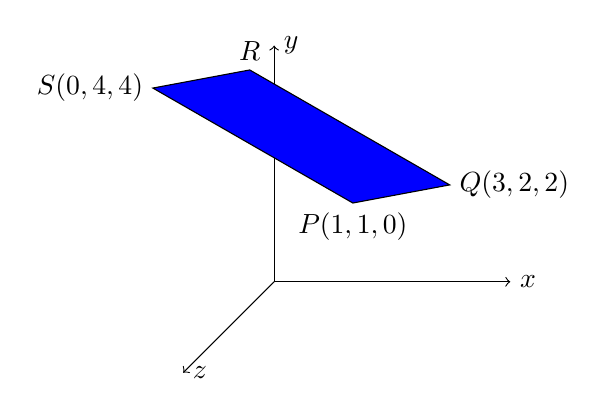
\begin{tikzpicture}
        % axes
        \draw[->] (0,0,0) -- (3,0,0) node[right]{$x$};
        \draw[->] (0,0,0) -- (0,3,0) node[right]{$y$};
        \draw[->] (0,0,0) -- (0,0,3) node[right]{$z$};
        \draw[fill=blue] (1,1,0) node[below]{$P(1,1,0)$} -- (3,2,2) node[right]{$Q(3,2,2)$} -- (2,5,6) node[above]{$R$} -- (0,4,4) node[left]{$S(0,4,4)$} -- cycle;
      \end{tikzpicture}
    \end{center}
    \begin{solution}
      The area is
      \[\begin{split}
        \|\overrightarrow{PQ}\times\overrightarrow{PS}\| &= \|(2,1,2)\times(-1,3,4)\| \\
        &= \|(4-6,-2-8,6+1)\|\\
        &= \|(-2,-10,7)\|\\
        &= \sqrt{153}\\
        &= 3\sqrt{17}.
      \end{split}\]
    \end{solution}

    \item Find the coordinates of point $R$.
    \begin{solution}
      The vector $\overrightarrow{PR}$ is equal to $\overrightarrow{PQ}+\overrightarrow{PS}$ by the parallelogram rule. So
      \[\overrightarrow{PR}=\overrightarrow{PQ}+\overrightarrow{PS}=(2,1,2)+(-1,3,4)=(1,4,6).\]
      Thus $R=P+\overrightarrow{PR}=(1,1,0)+(1,4,6)=(2,5,6)$.
    \end{solution}
  \end{enumerate}
\end{problem}

\begin{problem}
  Using vectors, we can prove that two lines in the $xy$-plane are perpendicular if their slopes multiply to $-1$.
  \begin{enumerate}[(a)]
    \item In the $xy$-plane, consider the line $y=mx+b$. Show that for any two points $P$ and $Q$ on the line, the vector $\overrightarrow{PQ}$ is parallel to the vector $(1,m)$.
    \begin{solution}
      First, an arbitrary point on the line $y=mx+b$ is obtained by choosing an arbitrary value $x=x_0$, after which $y$ must be equal to $mx_0+b$ by the equation.

      So let $P=(x_0,mx_0+b)$ and $Q=(x_1,mx_1+b)$ be arbitrary points on the line. The vector $\overrightarrow{PQ}$ is equal to $(x_1-x_0,(mx_1+b)-(mx_0+b))=(x_1-x_0,m(x_1-x_0))=(x_1-x_0)(1,m)$, which is a scalar multiple of $(1,m)$. This shows that $\overrightarrow{PQ}$ is parallel to $(1,m)$.
    \end{solution}
    \item Use part (a) to prove that if line $\ell_1$ is given by the equation $y=m_1x+b_1$ and $\ell_2$ is given by the equation $y=m_2x+b_2$, and if $m_1m_2=-1$, then $\ell_1$ and $\ell_2$ are perpendicular.
    \begin{solution}
      By part (a), the proposition that $\ell_1$ and $\ell_2$ are perpendicular is equivalent to the proposition that $(1,m_1)$ and $(1,m_2)$ are perpendicular vectors, because $\ell_1$ is parallel to $(1,m_1)$ and $\ell_2$ is parallel to $(1,m_2)$. Finally,
      \[\begin{split}
        (1,m_1)\perp(1,m_2) &\iff (1,m_1)\cdot(1,m_2)=0 \\
        &\iff 1+m_1m_2=0 \\
        &\iff m_1m_2=-1.
      \end{split}\]
    \end{solution}
  \end{enumerate}
\end{problem}

\begin{problem}
  The triangle inequality says that for all vectors $\bv$ and $\bw$,
  \[\|\bv+\bw\|\leq \|\bv\|+\|\bw\|.\]
  Of course I haven't proven it, but in part (b) of this problem you will prove it.
    \begin{enumerate}[(a)]
      \item Show that the triangle inequality holds for the example $\bv=(1,2)$ and $\bw=(-1,1)$.
      \begin{solution}
        The left hand side is equal to $\|(1,2)+(-1,1)\|=\|(0,3)\|=3$. The right hand side is equal to $\sqrt{5}+\sqrt2\approx 2.23+1.41=3.64$, which is greater than 3.
      \end{solution}
      \item Using the Cauchy-Schwarz inequality, prove the triangle inequality.
      \begin{solution}
        Let us prove the equivalent inequality $\|\bv+\bw\|^2\leq(\|\bv\|+\|\bw\|)^2$ instead. (Equivalent because both sides of the origial inequality are non-negative.) We have
        \[\begin{split}
          \|\bv+\bw\|^2 &= (\bv+\bw)\cdot(\bv+\bw)\\
          &= \bv\cdot\bv+2\bv\cdot\bw+\bw\cdot\bw\\
          &= \|\bv\|^2+2\bv\cdot\bw+\|\bw\|^2\\
          &\leq\|\bv\|^2+2\|\bv\|\|\bw\|+|\bw\|^2\qquad\text{(by Cauchy-Schwarz)} \\
          &=(\|\bv\|+\|\bw\|)^2.
        \end{split}\]
        \textbf{Remark}: Writing the right equations but without logically connecting them ends up being very hard to read and hard to follow for a reader. So it's important to format a proof in a coherent manner. For example, if it's one sentence long you can use a chain of equalities/inequalities as I did. Or you can write multiple statements, writing $\implies$ (``implies'') between two statements if the first one implies the other, or $\iff$ (``is equivalent to'') between two statements if the first one is equivalent to the second.

        With multiple statements which are logically connected, the proof is valid if and only if there exists a path of $\implies$ from the assumptions to the conclusion. For example, if you started from the conclusion and ended with an assumption, this is called a ``backwards proof'' and is typically invalid unless each statement is logically equivalent to the next (i.e.\ $\iff$, not just $\implies$).

        Notice that proofs in the textbook are never written as isolated lists of equations, for example.
      \end{solution}
  \end{enumerate}
\end{problem}

\begin{problem}
  Let $\bv=\mathbf j+\mathbf k$ and $\bw=\mathbf i+\mathbf j$.
  \begin{enumerate}[(a)]
    \item  Calculate $\bv\times\bw$ and verify that this cross product is perpendicular to both $\bv$ and $\bw$.
    \begin{solution}
      We can use any of the methods shown in class to calculate it. I'll show using distributivity, since it's probably the least common of the methods:
      \[\begin{split}
        \bv\times\bw &=(\bj+\bk)\times(\bi+\bj) \\
        &= \bj\times\bi+\bj\times\bj+\bk\times\bi+\bk\times\bj\\
        &= -\bk+\mathbf 0+\bj-\bi\\
        &= -\bi+\bj-\bk.
      \end{split}\]
      Let's calculate the dot products $(\bv\times\bw)\cdot\bv$ and $(\bv\times\bw)\cdot\bw$ and verify that they are both zero, which will tell us that $\bv\times\bw$ is perpendicular to both $\bv$ and $\bw$:
      \begin{align*}
        (\bv\times\bw)\cdot\bv &= (-\bi+\bj-\bk)\cdot(\bj+\bk)=(-1,1,-1)\cdot(0,1,1)=0+1-1=0,\\
        (\bv\times\bw)\cdot\bw &= (-\bi+\bj-\bk)\cdot(\bi+\bj)=(-1,1,-1)\cdot(1,1,0)=-1+1+0=0.
      \end{align*}
    \end{solution}
    \item Show that $\bv$ and $\bw$ are neither parallel nor perpendicular to each other.
    \begin{solution}
      The computation of the cross product in part (a) shows that $\bv\times\bw\neq\mathbf 0$, which proves that $\bv$ is not parallel to $\bw$, as the cross product of two parallel vectors is always $\mathbf 0$.

      Moreover, the dot product between $\bv$ and $\bw$ is $(0,1,1)\cdot(1,1,0)=0+1+0=1\neq 0$, which shows that $\bv$ and $\bw$ are not perpendicular.
    \end{solution}
    \item What is the component of $\bv$ in the direction of $\bw$? What is the component of $\bv$ perpendicular to $\bw$?
    \begin{solution}
      According to the clarification I gave on the website, I meant vector component for both parts. (Scalar component doesn't make sense for the part perpendicular to $\bw$ since I don't know whether to assign a positive sign or negative sign to the scalar component perpendicular to $\bw$.)

      The vector component of $\bv$ in the direction of $\bw$ is $\BP_\bw\bv=\frac{\bv\cdot\bw}{\bw\cdot\bw}\bw=\frac12\bw=(\frac12,\frac12,0)$.

      The vector component of $\bv$ perpendicular to $\bw$ is $\mathbf Q=\bv-\BP_\bw\bv=(0,1,1)-(\frac12,\frac12,0)=(-\frac12,\frac12,1)$.
    \end{solution}
    \item Show that there is no possible multiple of $\bw$ that can be added to $\bv$ to make the resulting vector parallel to $\bw$.
    \begin{solution}
      Yingying gave a nice solution using cross products.
      \begin{center}
        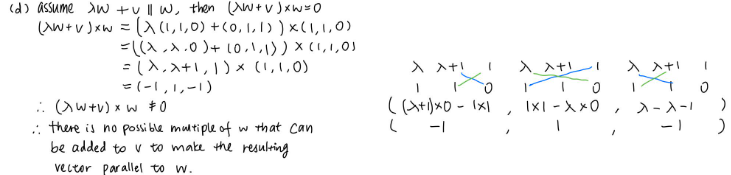
\includegraphics[width=\textwidth]{nice/p1.4c_yingying.png}
      \end{center}
      Most other people had the following valid solution by ``inspection'': If $\lambda$ is any scalar, then $\bv+\lambda\bw=(\lambda,1+\lambda,1)$, in particular, has $z$-coordinate 1. However, $\bw=(1,1,0)$, which has $z$-coordinate 0, implying that any scalar multiple of $\bw$ has $z$-coordinate 0. This implies that $\bv+\lambda\bw$ cannot be a scalar multiple of $\bw$.

      The following is the algebraic solution I had in mind: Suppose to the contrary that there exists $\lambda\in\bR$ such that $\bv+\lambda\bw=\mu\bw$ for some other scalar $\mu\in\bR$. Then $\bv=(\mu-\lambda)\bw$, which implies that $\bv$ is parallel to $\bw$. But we already know $\bv$ is not parallel to $\bw$, so this is a contradiction.
    \end{solution}
  \end{enumerate}
\end{problem}

\begin{problem}
  How difficult was each problem? Rate each problem (and part) on a difficulty scale from 1 to 7, where 1 means ``super easy, barely an inconvenience!'' and 7 means ``hardest problem I've ever done.''
\end{problem}

\newpage

\section{Hints}
\begin{hint}[for problem 1]
  The vectors $\overrightarrow{PQ}$ and $\overrightarrow{PS}$ may be important.

  Part (a) can be done after the lecture on cross products.

  Part (b) does not need the lecture on cross products, but you may want to recall the parallelogram law for vector addition as shown in Figure 7 in p.724.
\end{hint}

\begin{hint}[for problem 2]
  For (a), show that an arbitrary point on $y=mx+b$ can be represented by the ordered pair $(x_0,mx_0+b)$.
\end{hint}

\begin{hint}[for problem 3(b)]
  A good first step is to square both sides of the equation and then rewrite $\|\bv+\bw\|^2$ as $(\bv+\bw)\cdot(\bv+\bw)$.
\end{hint}
